% This is the Reed College LaTeX thesis template. Most of the work
% for the document class was done by Sam Noble (SN), as well as this
% template. Later comments etc. by Ben Salzberg (BTS). Additional
% restructuring and APA support by Jess Youngberg (JY).
% Your comments and suggestions are more than welcome; please email
% them to cus@reed.edu
%
% See http://web.reed.edu/cis/help/latex.html for help. There are a
% great bunch of help pages there, with notes on
% getting started, bibtex, etc. Go there and read it if you're not
% already familiar with LaTeX.
%
% Any line that starts with a percent symbol is a comment.
% They won't show up in the document, and are useful for notes
% to yourself and explaining commands.
% Commenting also removes a line from the document;
% very handy for troubleshooting problems. -BTS

% As far as I know, this follows the requirements laid out in
% the 2002-2003 Senior Handbook. Ask a librarian to check the
% document before binding. -SN

%%
%% Preamble
%%
% \documentclass{<something>} must begin each LaTeX document
\documentclass[12pt,twoside]{reedthesis}
% Packages are extensions to the basic LaTeX functions. Whatever you
% want to typeset, there is probably a package out there for it.
% Chemistry (chemtex), screenplays, you name it.
% Check out CTAN to see: http://www.ctan.org/
%%
\usepackage{graphicx,latexsym}
\usepackage{amssymb,amsthm,amsmath}
\usepackage{longtable,booktabs,setspace}
\usepackage{chemarr} %% Useful for one reaction arrow, useless if you're not a chem major
\usepackage[hyphens]{url}
\usepackage{rotating}
\usepackage{natbib}
\usepackage{listings}
\usepackage{tikz}
\usepackage{algorithm}
\usepackage[noend]{algpseudocode}

\lstset
{ %Formatting for code in appendix
	basicstyle=\footnotesize,
	numbers=left,
	stepnumber=1,
	showstringspaces=false,
	tabsize=4,
	breaklines=true,
	breakatwhitespace=false,
}

% Comment out the natbib line above and uncomment the following two lines to use the new
% biblatex-chicago style, for Chicago A. Also make some changes at the end where the
% bibliography is included.
%\usepackage{biblatex-chicago}
%\bibliography{thesis}

% \usepackage{times} % other fonts are available like times, bookman, charter, palatino

\newcommand{\ceil}[1]{\lceil #1 \rceil}
\newcommand{\floor}[1]{\lfloor #1 \rfloor}

\title{My Final College Paper}
\author{Your R. Name}
% The month and year that you submit your FINAL draft TO THE LIBRARY (May or December)
\date{May 200x}
\division{Mathematics and Natural Sciences}
\advisor{Advisor F. Name}
%If you have two advisors for some reason, you can use the following
%\altadvisor{Your Other Advisor}
%%% Remember to use the correct department!
\department{Mathematics}
% if you're writing a thesis in an interdisciplinary major,
% uncomment the line below and change the text as appropriate.
% check the Senior Handbook if unsure.
%\thedivisionof{The Established Interdisciplinary Committee for}
% if you want the approval page to say "Approved for the Committee",
% uncomment the next line
%\approvedforthe{Committee}

\setlength{\parskip}{0pt}
%%
%% End Preamble
%%
%% The fun begins:
\begin{document}

  \maketitle
  \frontmatter % this stuff will be roman-numbered
  \pagestyle{empty} % this removes page numbers from the frontmatter

% Acknowledgements (Acceptable American spelling) are optional
% So are Acknowledgments (proper English spelling)
    \chapter*{Acknowledgments}
	I want to thank a few people.

% The preface is optional
% To remove it, comment it out or delete it.
    \chapter*{Preface}
	This is an example of a thesis setup to use the reed thesis document class.



    \chapter*{List of Abbreviations}
		You can always change the way your abbreviations are formatted. Play around with it yourself, use tables, or come to CUS if you'd like to change the way it looks. You can also completely remove this chapter if you have no need for a list of abbreviations. Here is an example of what this could look like:

	\begin{table}[h]
	\centering % You could remove this to move table to the left
	\begin{tabular}{ll}
		\textbf{ABC}  	&  American Broadcasting Company \\
		\textbf{CBS}  	&  Columbia Broadcasting System\\
		\textbf{CDC}  	&  Center for Disease Control \\
		\textbf{CIA}  	&  Central Intelligence Agency\\
		\textbf{CLBR} 	&  Center for Life Beyond Reed\\
		\textbf{CUS}  	&  Computer User Services\\
		\textbf{FBI}  	&  Federal Bureau of Investigation\\
		\textbf{NBC}  	&  National Broadcasting Corporation\\
	\end{tabular}
	\end{table}


    \tableofcontents
% if you want a list of tables, optional
    \listoftables
% if you want a list of figures, also optional
    \listoffigures

% The abstract is not required if you're writing a creative thesis (but aren't they all?)
% If your abstract is longer than a page, there may be a formatting issue.
    \chapter*{Abstract}
	The preface pretty much says it all.

	\chapter*{Dedication}
	You can have a dedication here if you wish.

  \mainmatter % here the regular arabic numbering starts
  \pagestyle{fancyplain} % turns page numbering back on

%The \introduction command is provided as a convenience.
%if you want special chapter formatting, you'll probably want to avoid using it altogether

% The three lines above are to make sure that the headers are right, that the intro gets included in the table of contents, and that it doesn't get numbered 1 so that chapter one is 1.

% Double spacing: if you want to double space, or one and a half
% space, uncomment one of the following lines. You can go back to
% single spacing with the \singlespacing command.
% \onehalfspacing
% \doublespacing


\chapter*{Introduction}
\lstset{language=C++}
\addcontentsline{toc}{chapter}{Introduction}
\chaptermark{Introduction}
\markboth{Introduction}{Introduction}

	\section{Overall motivation}

		In the heterogeneous computing world, there are tools to create software for specific devices. There are also languages which can compile to many different devices (e.g. OpenCL). However, the number of devices is growing, and their characteristics are getting further apart. There will probably never be one language which works for all devices, and all problems. And there is certainly not one available now. So programmers have to write code for different kinds of devices, so that their application can run efficiently. However, programmers have to rely on their knowledge and intuition to figure out what sorts of hardware is appropriate for their application. As the number of different hardware platforms keeps on growing, this puts more and more strain on software developers to become knowledgeable about all sorts of hardware.

		To solve this problem, we suggest making a tool, which can examine CPU code run on a typical workflow, and output suggestions of what kind of hardware different parts of the code can run on.

		This will allow programmers to focus on the hardware platform that is most useful to them reducing search cost. They will still need to learn how to program that hardware, and make their code run efficiently, but at least they will not d all that work to find out that they chose the wrong hardware.

		\subsection{General areas of use cases}

		\subsubsection{Performance-Generality tradeoff}

		General purpose hardware to improve performance is fairly limited in scope. GPUs are broadly understood by the performance programming community, and more accessible tools are improving at a great pace. FGPAs are quickly catching up. And other coprocessors, like Audio and Encryption accelerators seem to lack proper enough generality to be useful in broad cases [CHECK IF THIS IS ACTUALLY TRUE, LOOK FOR PEOPLE WHO HAVE TRIED TO DO THIS!!!!!!!!!!!!!!!!!!!!!!!!!!!!!].

		This is because the tradeoff between generality and performance, which has few points since the software efforts to adopt new hardware is too great to justify too many points.

		One possible use case is reducing the cost of adding more points to this curve. If people can match code to hardware capabilities easily, then the search cost of finding the right parts of the software and finding the right parts of the hardware can be reduced. Lowering the cost of changes along this curve can increase granularity, and perhaps bring a new wave of slightly less general hardware. [TALK ABOUT EITAN'S SMART NICs]

		However, while this use case is intriguing in theory, in practice, it will change nothing until people are already using it,  which is unlikely if it is not very useful. So we need to look for other useful.

		\subsubsection{Power-Performance tradeoff}

		Perhaps the most useful application of this design is helping programmers understand how different hardware platforms will impact power consumption.

		Performance and generality have clear tradeoffs. But when you throw in power into the mix, the hardware world becomes much more daunting.

		In power, the hardware can simply adopt similar software interfaces, but have dramatically different

		\footnote{\cite{Taylor:2013}}

		There are a wide variety of new hardware

		%\subsection{Mainstream approach}

		%Right now, people face the tradeoff between performance and productivity as a fact of life. Except for GPUs, which have mature high level languages, adopting a new hardware platform usually means

		%The reality is that the vast majority of software does not see heterogeneous computing as a viable option. Of course, machines are fast enough that we don't have to worry about most software, only ones that consume lots of resources.

		%So what kinds of software are we looking to help?

		%The advance of scripting languages such as Python, Ruby, and Javascript means that most modern code is running much slower than it could be if written in a more performance centric language, and so improvements in software can dramatically improve performance and power with no changes to hardware. This is the extreme "productivity" side of the tradeoff,  and there is little we can do here.

		%But the advance of these scripting languages also has brought fast CPU-GPU libraries to exploit various hardware platforms. This is a dominant paradigm in scientific computing.

		%The best supported and most popular libraries, like BLAS, have separate implementations for every imaginable hardware platform. This is the extreme "performance" side of the tradeoff, and again, there is little we can do.

		%\subsection{Best approach (mainstream among theorists)}

		%Right now, academics see the most promising route to be changing software models.

		%Existing cross heterogeneous computing languages and paradigms, such as OpenCL, struggle with "performance portability." This means that when the programmer tries to run the code on new hardware, it may run much worse than the original hardware. [CITATION!!!!!!!!!!!!!!!!!!!!!!!!!!!!!]

		%\subsection{Improving mainstream approach}


	\subsection{Note about workload characterization}

		A related field of research is workload characterization. The purpose here is to examine how real software runs on hardware, with the purpose of improving the hardware to run the software faster.

		Our work is related since both fields of study are interested in how real software performs on hardware, what sorts of software can run on what sorts of hardware. This means we will use tools originally intended for workload characterization, particularly binary instrumentation tools.

		However, the fields have a fundamentally different purpose. We are making a tool to help inform a software developer working with a particular software project about the many different kinds of hardware available. Workload characterization is fundamentally making a tool for the hardware developer, working with a particular piece of hardware, and informing them about the many different types of software.

		This fundamental difference will mean that we cannot copy over the same techniques. In particular, hardware developers have to assume that software runs well “as is” as they cannot hope to improve it. However, software developers can change their software to fit the hardware better. So we need to be much more open to changes in the order of execution of parallel instructions, for example, as they will certainly change when moving from CPU to GPU.

		It seems to me at first glance that this will mean that we need much more complete information about the program than the summary statistics that workload characterization researchers use.

		Two examples I can think of right now are:

		\begin{enumerate}
			\item SIMD instruction size: We need to know if the SIMD size expressed by the cpu code is optimal, or if it can be substantially increased by minor changes to the code. This may be the difference of porting it to GPU improving performance or not

			\item Level of parallelism. It is kind of difficult to find natural parallelism in arbitrary code to begin with. But when you consider that certain operations (like reductions) are implemented in a highly sequential manner in single threaded programs, but can be rewritten to run in a massively parallel manner. So ideally, we should be able to figure out if they can be written in this way.  (perhaps by keeping track of associative operations)
		\end{enumerate}

		\subsection{Note about Intel\textsuperscript{\textregistered} Advisor}

		Intel advisor is a very similar tool to what we are using. It's goal is to tell the programmer how they should go about vectorizing and threading their code. This tool can be very effective for both Intel CPUs and Intel Xeon Phi Coprocessors.

		Our end goals are quite separate. Intel's goal is to create an interactive workflow that continuously profiles code on the machine as you optimize it. This is impossible for our purposes, as we will only instrument CPU binary code (this is the only code Intel cares about), and not the code of the machine we are interested in making inferences about.

		But this goal is super important in its own right, and there does not appear to be an open source alternative to intel's tools right now.

		One use case goes like this:

		\begin{enumerate}
			\item
			You are developing code for a system, you profile the code and you find a performance critical section.
			\item You use our tool to understand if this section of code can be parallelized, and what kind of parallelization it can handle (vector, thread, or both).

			\item If the tool tells you it can be parallelized, and what kind, this will allow you to confidently spend time on this code knowing that it will be worth it.

			If the tool tells you it can't be parallelized, then it should give you some indication about why it can't be, and where in the code the problem is arising.

			This should allow the programmer to determine if there is some workaround for the problem.

			possible problems/fixes:

			\begin{enumerate}
				\item Problem: Critical data dependency:

				Possible solution: Perhaps there is an algebraic or algorithmic trick that allows you to parallelize it.

				\item Problem: side data dependency (dependency occurs in a logger, assert, or some other non-critical code)

				Possible solution: There is usually some workaround here. In the worst case, you can just remove the non-critical code.

				\item Data strides of more than 1 (hurts vectorization):

				Possible solution: This can usually be optimized somehow, although sometimes the solution is not trivial.

				\item Non-regular access (vector issues). Similar to previous one, except even less likely to succeed, and even more non-trivial.
			\end{enumerate}

		\end{enumerate}

		Note that while this is useful for developing faster code for a single system, it is also necessary to properly use our tool. Parallelism is a critical input to the analysis, and if it is wrong, because of some minor error that can be fixed easily, then you need to fix it before running the analysis, or else it will make a mistaken analysis.

		And the Intel advisor code involved is very proprietary, and the tools are very expensive (starts at \$1600), and it is not built to be useful for non-Intel processors, or even Intel Integrated Graphics, so it will not be very helpful to achive our goals.

		So we need some sort of analysis separate from Intel Advisor, but which allows for a similar workflow.

	\section{Parts of thesis}

		This thesis has several different parts. Although they also build to a single core purpose, they also have other interesting connections, inspirations and applications.


		High level implementation description

		There will be several parts

		Tool which extracts basic runtime information from actual running code (dependencies, memory addresses, instruction type)
		Library which takes basic info from tool and converts it into hardware properties (vector sizes, pipeline sizes, parallelism)
		Library which converts hardware properties into advice about hardware


	\subsection{Parallelism detection}

		\subsubsection{Applications of parallelism detection}

		Parallelism detection is super useful for many different applications.

		People have suggested using it for determine where to make speculative automatic parallelization. \footnote{\cite{Chen:2004}} There idea here is that the compiler may not be able to prove that the code is parallel, but it may be able to generate code where if there is not a data conflict, or not many, then there is minimal performance loss. Of course, if there are many dependencies, there may be significant performance loss, so the profiler needs to establish a high degree of parallelism on real inputs.

		It is also useful in a tool which tell the software developer what is parallelizable and what is not.[CITATION!!!!!!!!!!!!!!!!!!!!!!!!!!!!!!!!!!!!!]
		In larger, complex software, often dependencies are not clearly defined, and manually determining dependencies by sifting through code may be impractical. But dynamic dependency analysis will tell the developer for sure if a block of code can be safely parallelized on the inputs given (it guarantees nothing about other inputs, but this test may be good enough for many developers).

		Then, of course, it is critical for our goal. The common theme among new architectures is trading off single threaded performance for power efficiency or high degrees of parallelism [CITATION!!!!!!!!!!!!!!!!!!!!!!!!!!!!!!].
		So determining whether it can exploit parallelism is critical to establishing whether the decrease in sequential performance is will be sufficiently offset by improved parallelism.

		So we need to detect parallelism. How do we go about doing this? (Chapter 1)

	\subsection{binary instrumentation}
		\footnote{\cite{Luk:2005}}

	\subsection{Hardware identification}

	\subsubsection{Things we should consider from software side}


	\begin{itemize}
		\item Parallelism  (whole section on that)
			\begin{itemize}
			\item Instruction parallelism (super-scalar vs sequential)
			\item Data parallelism
			\item Thread parallelism
			\item Reductions
			\end{itemize}

		\item Memory access pattern
			\begin{itemize}
			\item is it random
			\item does it allow for vector operations
			\item how many 4k blocks does it touch
			\item Does it stride
			\end{itemize}

		\item Instruction composition
			\begin{itemize}
			\item Lots of floating points operations?
			\item Complex integer functions (div,mul) vs simple ones (add, lea)?
			\item
			\end{itemize}

		\item Code pattern
			\begin{itemize}
			\item Do branches taken in a loop diverge? If so, maybe not GPU, if not, then maybe GPU is good.
			\item Is there non-trivial recursion or random access code pointers? If so, then many processors like GPUs will not work.
			\end{itemize}

	\end{itemize}


	\subsubsection{Things we should consider from hardware side}

	\begin{itemize}
		\item Power vs performance need of software (user input)

		\item Overhead from shifting between processors:

		The big problem is that shifting data across different processors, and telling those processors to do things with that data takes a significant amount of overhead. With GPUs, this can take milliseconds (source).

		\item Superscalar pipelines/dispatch

		\item Degree and levels of parallelism in hardware

		\item Cache sizes/ hierarchy/ local-shared memory/

	\end{itemize}

\chapter{Dynamic parallelism detection}

	\section{Introduction}
		We need a way of determining parallelism in order to do any useful inference on hardware compatibility. But, also recall that our end goals are much larger than just that. We are looking at a wide vision of a tool that helps the programmer understand their code, and help them to improve the algorithms and prototype them for better fitness on different hardware without actually dealing with the hardware. So we not only want a parallelism tool that figures out which parts of the code can be parallelized or not, but a tool that helps the programmer understand why code might not be parallelizable, and perhaps how to fix it. 
		 
		We came to the conclusion that current open source parallelism detection tools do not meet our efficiency and accuracy requirements, and so we built our own tool which does meet our needs. 
		
		This chapter goes over the necessary background for that tool. In section 2, we introduce the type of parallelism we are detecting, and why it is so important. In section 3, we introduce the base algorithm for detecting it, and the problems with it. In section 4, we go over prior work in this area, and how it doesn't suit our needs completely. 
		
	\section{Loop level parallelism}
	
		Parallelism is a general topic that can apply to all sorts of code in all sorts of ways. We will only be discussing a very specific kind of parallelism: loop level parallelism (LLP). This type of parallelism is common, easy to detect, scales well on massively parallel hardware, and simple for programmers to reason about. 
		
		But before we get into the details of why we care so much about loop level parallelism, lets go into some detail about what it is.
		
		\subsection{What is Loop level parallelism?}
		
		In a vague sense, LLP occurs when each iteration of the loop can be run in parallel with all the other iterations. 
		
		Here is a vector-scalar multiply procedure. 
		
		\begin{lstlisting}
for(int i = 0; i < n; i++){
	B[i] = B[i] * 2;
}
		\end{lstlisting}
		
		The above loop is parallel because every iteration is independent from every other iteration. In other words, you can compute this loop given any ordering of \texttt{i}.
		
		Here is a cumulative sum algorithm. 
		
		\begin{lstlisting}
for(int i = 1; i < n; i++){
	B[i] = B[i-1] + A[i];
}
		\end{lstlisting}
		
		This procedure is not loop-parallel. It needs to compute \texttt{B[i-1]} before it can calculate \texttt{B[i]}. 
		
		\subsection{Desirable qualities of loop level parallelism}
		
		We like LLP for four reasons: it is common, scales well on massively parallel hardware, simple for programmers to reason about, and easy to detect. 
		
		Of course, loops are very common in all low level code. A large number of these loops are loop parallel. 
		
		Loop level parallelism is part of a class of parallelism called massive parallelism That means that if the loop is reasonably large, it can be scaled to massively parallel hardware like GPUs or other kinds of accelerators. 
		
		Parallelizing loops is also very simple for the programmer to reason about. With OpenMP, one can parallelize loops on CPUs with a one line directive. In lower level accelerator code, like OpenCL, it is still relatively easy to translate loops into parallel kernels, just by porting the inner part of the code to an kernel, and run it on all the iterations of the loop in parallel 
		
		Lastly, loop level parallelism is easy to detect. The next section will give a simple algorithm to detect this. Other kinds of massive parallelism require more sophisticated analysis. 
		
		\subsection{Dynamic Loop Detection}
		
		Loops have a clean structure in high languages like C. However, as we are interested in doing dynamic profiling that will require us to understand the structure of loops in machine code. And loops in machine code are simply difficult to work with, as they are implemented with "go to" instructions which happen to go back to where you came from, rather than somewhere else. So in order to understand loops in machine code, we have to somehow separate loops out from a tangle of "go to" instructions. 
		
		Luckily, there is prior work for doing just this. We use LoopProf \footnote{\cite{Chen:2004}} code in order to detect locations of loops in code. In particular, LoopProf tells us where the loop begins, and the nesting structure of the loops. However, the LoopProf implementation did not contain all of the functionality we needed. In particular, it did not detect precise ends of loops, which we needed for dynamic dependence analysis. So we made some alterations in order to deal with this problem. Unfortunately, these are technical enough and far enough away from the point of this chapter, that we will not get into more detail about this. 
		
	\section{The baseline algorithm: The pairwise method}
	
		Our goal is to build an efficient algorithm for determining parallelism of loops and tracking where dependencies are in code. We will introduce a simple method which can gather then necessary information, and then optimize it using compression. This simple method is called the pairwise method. 
		
		Before diving into details, we'll give a broad overview of the concepts behind the pairwise method. All of this will be explained in more detail later. 
		
		
		Recall that loop parallelism occurs when each iteration of loop can be executed independently from every other iteration, and that independence means that one iteration doesn't depend on data computed by another iteration. 
		The pairwise method tracks dependencies as reads and writes to memory. Each read is considered to be an input to the computation in the loop, and each write is an output. So if one loop iteration reads from one bit of memory and a later one writes to that same byte of memory, then that is a dependence that should be recorded. 
		
		Now, there is an importance difference between memory and dependencies. Memory can sometimes be reused without creating dependencies. In particular, if memory is written to before it is read in a loop iteration, then it is "cleared", and further reads in that iteration will not be tracked for dependencies. 
		
		So we will store 3 things:
		
		\begin{itemize}
			\item history table: A table of reads and writes of previous loop iterations.
			\item pending table: A table of reads and writes of the current loop iteration
			\item killed bits: A set of instructions which were written before read in the current loop instance. 
		\end{itemize}
	
		All of this becomes more clear with examples.
		
		
		
		\subsection{Simple demonstration}
		
		Here is the cumulative sum procedure, written in terms of reads and writes
		
		\begin{lstlisting}
for(int i = 1; i < n; i++){
	READ B[i-1]
	READ  A[i]
	WRITE B[i]
}
		\end{lstlisting}
		
		Here is the state of the history and pending tables at the end of the 3rd loop iteration. 
		
		\begin{tabular}{ |c|c|c| } 
			\hline
			\multicolumn{3}{|c|}{Pending Table} \\
			\hline
			Instr & Memory & R/W \\ 
			\hline
			2 & B[2] & R \\ 
			3 & A[3] & R \\ 
			4 & B[3] & W \\ 
			\hline
		\end{tabular}
		\begin{tabular}{ |c|c|c| } 
			\hline
			\multicolumn{3}{|c|}{History Table} \\
			\hline
			Instr & Memory & R/W \\ 
			\hline
			2 & B[0] & R \\ 
			3 & A[1] & R \\ 
			4 & B[1] & W \\ 
			2 & B[1] & R \\ 
			3 & A[2] & R \\ 
			4 & B[2] & W \\ 
			\hline
		\end{tabular}
		
		
		
		\subsection{Nested loop demonstration}
		
		Now, this method also needs to work for nested loops.  
		
		In this vector-matrix multiplication procedure, the inner loop is not parallel, but the outer loop is. We need to be able to detect this.
		
		
		\begin{lstlisting}
for(int i = 0; i < output_size; i++){
	y[i] = 0
	for(int j = 0; j < input_size; j++){
		y[i] += M[i][j] * x[j]
	}
}
		\end{lstlisting}
		
		When \texttt{i = 2} and \texttt{j = 2}, the resulting table looks like:
		
		
		
		\subsection{Registers/Stack}
			
			
	\section{Motivation}
	
		Recall that one of the most important things to establish about the program is whether it can in theory run in parallel. This is a very important factor in determining a program's hardware matchup.

		One problem is that there are no good open source tools for determining theoretical parallelism in real code. So we will have to create one ourselves. We will constrain ourselves to loop parallelism, as detecting general parallelism is impossible. 
		
		To help explain the algorithms and data structures involved, I will bring in a couple of code examples in order to show how the algorithms work. 
		


	\section{Data Dependency graphs}
		So how might you detect parallelism? To do that, you have to have a mathematical model of what parallelism is.

		Our model is a data dependency graph.

		The idea is that we can take a computation and build a directed acyclic graph like so.

		The inputs to the computation are nodes $I \subset V$. These can be thought of as blocks of memory stored before the computation starts. Each step of the computation produces a temporary value $c \in V$. There is an edge $(u,v)$ whenever an input to $u$ is the data calculated by $v$. Then some nodes are designated outputs, which are the data we wished to calculate.

		This is a directed acyclic graph because in a computation, no sub-computation can use data that hasn't been calculated yet, including the data output by its own computation.

		For example, you can break the computation of $A+B+D+A\times B$ into a few steps like this

		\begin{algorithmic}[1]
			\State $D \gets A+B$
			\State $E \gets A\times B$
			\State $F \gets D+C$
			\State $G \gets E+F$
		\end{algorithmic}

		And then use these sub-operations to build the following dependency graph.

		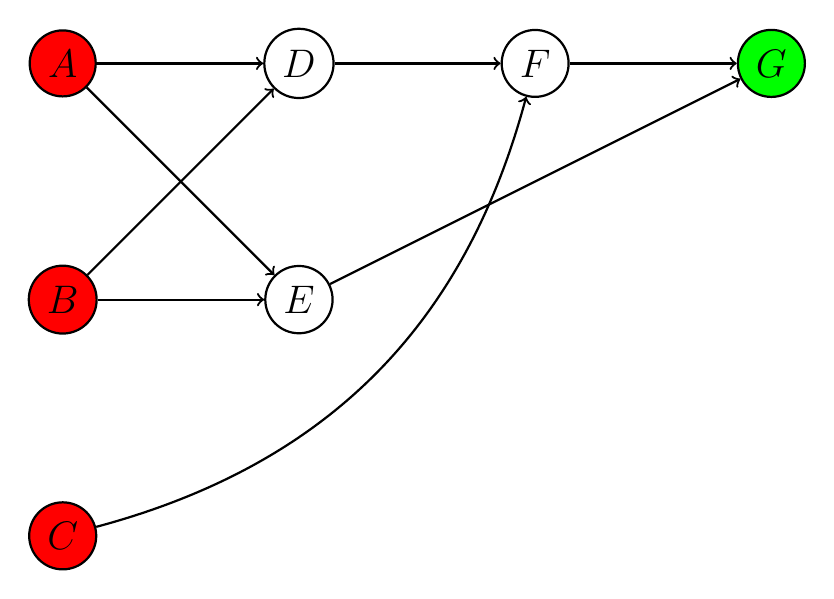
\begin{tikzpicture}[auto, node distance=3cm, every loop/.style={},
		thick,main node/.style={circle,draw,font=\sffamily\Large\bfseries}]

		\node[main node] [fill=red] (A) {$A$};
		\node[main node] [fill=red] (B) [below of=A] {$B$};
		\node[main node] (C) [right of=B] {$E$};
		\node[main node] [fill=red] (D) [below of=B] {$C$};
		\node[main node] (F) [right of=A] {$D$};
		\node[main node] (E) [right of=F] {$F$};
		\node[main node] [fill=green] (G) [right of=E] {$G$};

		\path[every node/.style={font=\sffamily\small}]
		(A) [->] edge node [left] {} (C)
		(B) [->] edge node [left] {} (C)
		(A) [->] edge node [left] {} (F)
		(B) [->] edge node [left] {} (F)
		(F) [->] edge node [left] {} (E)
		(E) [->] edge node [left] {} (G)
		(C) [->] edge node [left] {} (G)
		(D) [->] edge [bend right] node [left] {} (E);
		\end{tikzpicture}

		Hopefully you can see that this is an intuitive framework to examine parallelizability In the example above, nodes $D$ and $E$ can be run in parallel since neither depend on the other. $F$ can also be run in parallel with $E$, but not with $D$, since it depends on $D$ already being calculated. $G$ can only be run after all other steps are finished, as it recursively depends on $D,E$, and $F$.

		The degree to which this graph is parallelizable corresponds to the depth of the graph. By depth, we simply mean the maximal length of any path from an input to an output. This can be easily calculated using topological sort. This maximal length is guaranteed to be finite for any directed acyclic graph. In the example above, the depth is 3, as $A\rightarrow D \rightarrow F \rightarrow G$ has 3 edges, and no path has more than 3.

		The most important kind of parallelism, and the only kind we will care about is massive parallelism. Massive parallelism is defined to be any computation where the depth of the dependency graph is logarithmic in the size of the input.

		One extremely simple example of a massively parallel algorithm is a vector addition. If you want to sum two vectors $a$ and $b$, by computing $c = a+b$, then the obvious algorithm is to take each $i$, and compute $c_i = a_i + b_i$. Since each of these operations is completely dependent on the others, this is a constant depth dependency graph.

		One important example of a massively parallel algorithm is summing. When you have an array $A_1,A_2,...,A_n$ of numbers and you sum them, there are different ways to do it, some of which are parallelizable, some of which are not. The most obvious sequential algorithm, computing $(A_1+(A_2+(A_3+...+A_n)))$ has a dependency graph of depth $n$. However, addition is associative, so we can rearrange the parenthesis like this: $(((A_1+A_2)+(A_3+A_4))+...(A_{n-1}+A_n))$ to give us a log depth dependency graph. Below are two algorithms that describe these methods.

		\begin{algorithm}
			\caption{MassiveParrelelSum}\label{parellelsum}
			\begin{algorithmic}[1]
				\Function{RecursiveSum}{A,s,e}
					\If {$e - s \le 2$}
						\Return {$\textsc{StandardSum}(A[s:e])$}
					\EndIf
					\State $m \gets \floor{e-s}$
					\State $s_1 \gets \textsc{RecursiveSum}(A,s,m)$
					\State $s_2 \gets \textsc{RecursiveSum}(A,m,e)$
					\State \Return $s_1+s_2$
				\EndFunction
				\Function{StandardSum}{A}
					\State $s \gets 0$
					\For{$a \in A$}
						\State $s \gets s + a$
					\EndFor
				\EndFunction
			\end{algorithmic}
		\end{algorithm}

		Now, this is bad since we have two algorithms to compute the same problem, but one of which is parallelizable, and one of which is not. And what allows us to do the transformation from one to the other depends on an algebraic quality that is true for many operations and procedures other than addition. For example subtraction is not associative, but repeated subtraction can have a similar transformation because you can take $\text{RepeatedSubtraction}(A) = -\text{Sum}(A)$, and then do the same log depth calculation with only one more step at the end.

		This general method of using divide and conquer to turn a linear depth operation into a log depth one is called a reduction, and is the basis of the MapReduce cluster computing paradigm.

		Since these are important targets of parallelization, we will try our best to identify these cases, but it is most likely impossible to assess the possibility of this transformation automatically with perfect accuracy, so we will have to analyses actual cases.

		\subsection{Reporting}

		Just detecting a binary "is parallel" or "is not parallel" is not particularly useful. If it is a small loop, then it is easy to see if it is parallel or not by hand. A larger loop in real code is quite unlikely to have no data dependencies at all, and so they will rarely be parallel. If the parallelism detector says a larger function is not parallel, then the analysis you do with it won't know if the part that is not parallel is important or not. It could be an assert or logging that is non-vital, or perhaps something that can be pulled out of the loop. However, it is difficult to automatically detect such things, but instead, we can report what in the loop is stopping the function from being parallel to a human. A human, one shown where the problems are, may be able to tell  And a human using this tool won't know where the problem is, and may take a lot of work to find this issues, unless the code tells the human where to look. The most useful information is what instruction the conflicts are coming from, but there are others, for example, the memory location, and the number of accesses which conflict.

		The number of times conflicting accesses happen is useful for us because it gives some indication as to how well it were to perform if we had some sort of locking mechanism serializing accesses to the bit of memory.

		Because this is not the main point of the thesis, I will focus on making a good attempt to report the instruction locations of the conflict, and the number of times conflicts happen. But perfection is not necessary here.

		\subsubsection{Reporting List}
		\begin{enumerate}
			\item Whether a loop is parallel
			\item Number of bytes that conflict between iterations
			\item Instructions that conflicts
			\item etc.
		\end{enumerate}

	\section{Pairwise method}

		Note that any naive implementation of actually constructing a data dependence tree from a real computation will take $\Omega(n)$ space, where $n$ is the number of steps of the computation. Even for quick computations, this memory requirement quickly grows beyond RAM capacities of normal machines, and analysis becomes unusably slow. So instead, we will look at special cases and approximations to get what we need.

		The pairwise method is a approximation of data dependence analysis which has been developed to examine loop level parallelism.

		\subsection{Terminology}
		\begin{itemize}
			\item Loop iteration
			\item Loop instance
		\end{itemize}

		\subsection{Idea and inspiration}

		Loop level parallelism is when one iteration of a loop is independent from the rest. This kind of parallelism is the main target of massively parallel architectures. Other types of parallelism, including parallel recursive calls and task parallelism are generally less important or less parallelizable than loop level parallelism.

		The idea is to figure out if an iteration of a loop is independent from each other loop iteration. If this is the case, then it clearly is highly parallelizable

		The real reason why this is an important case is because it is very easy to measure, requiring very little memory and computation. Take the following loop:
\begin{lstlisting}
for(int i = 1; i < n; i++){
	//operation 1
	//operation 2
	//operation 3
	//...
}
\end{lstlisting}


		To check if this code runs in parallel, we only need to keep track of two things:

		\begin{enumerate}
			\item Which memory addresses have been written and read in the current loop iteration. Call this the pending table.
			\item Which memory addresses have been written and read in all of the previous loop iterations in the same instance. Call this the history table.
			\item Which memory addresses in the current loop iteration that their first access was a write. Call this the killed addresses.
		\end{enumerate}

		So int the example above, say we were at operation 2 in iteration 30. So in other words, $i=30$, and we have executed operation 1.

		Then we only need to keep track of which memory addresses were read and written in operation 1 in the current iteration, and the reads and writes of all the operations in each previous iteration, i.e. when $i < 30$.

		So instead of having a memory requirement that scales with the size of the number of operations in the code, we have a memory requirement proportional to the amount of memory that the original app uses times the number of nested loops.

		\subsection{Implementation}

		The algorithm itself is quite simple:

		You just need 4 core operations, and the rest is straightforward:

		\begin{enumerate}
			\item Add a new memory access to the pending tables, considering killed bits of current loop iteration
			\item Merge in the historytable from a nested loop into the pendingtable of the current loop. When doing so, remove the killed addresses, and add the addresses that have been written to the killed addresses set.
			\item Merge in pending table into history table, finding access conflicts between the two.
		\end{enumerate}

		\begin{algorithm}
			\caption{Pairwise-Method}\label{pairwise-method}
			\begin{algorithmic}[1]
				\State When you see a new loop, push it on the loop stack
				\State On memory access, \textsc{ADD}
				\State On loop iteration end \textsc{MERGE PEND HIST}
				\State On loop instance end \textsc{MERGE HIST PEND}
			\end{algorithmic}
		\end{algorithm}

		\subsection{Correctness}

		To prove that this always produces a correct answer to the problem, consider the each loop iteration to be a single computation in the graph. The memory addresses that are reads first are clearly inputs to this operation, and the output are writes. Memory addresses that are written before being read are not inputs, and so should not be counted as such.

		So if any write of one iteration is read by another, then clearly, this dependency graph is not 1 depth, as the output of one operation is the input of another.

		If the dependency graph is depth 1, then this means there was no reads of any data that was output in other iterations.

		So this method works if every loop is independent from every other loop.

		Unfortunately, this method does not guarantee any good results if there is any dependence whatsoever in between loops for example, the following loop has a dependency graph depth of two.

\begin{lstlisting}
for(int i = n; i < 3n; i++){
	A[i] = A[i-n]+1;
}
\end{lstlisting}

		To see why its dependency graph is so small, note that you can simply break this into two loops, one from $i = [n,2n-1]$, and $i=[2n,3n-1]$, and in both loops, simply compute the answer in parallel.

		However, the pairwise method simply returns that all of the iterations after $i \ge 2n$ are not parallelizable, as they conflict with the memory addresses in some previous iteration. This is a direct consequence of the memory saving property of the pairwise method, so this problem is not solvable by this method.

		\subsection{Collecting additional information}

		As mentioned before, we will want not only report a binary parallel/not parallel, but also collect some fairly substantial additional information. In particular, we care about which instruction the dependencies came from.

		So in addition to storing information about which memory accesses are reads and writes, we will also need to store the instruction each read and write came from. One way to implement this is to store a set of memory reads and writes for each instruction.
%\begin{lstlisting}
%for(int i = 0; i < n; i++){
%	B[i] = A[i-1];
%	A[i] = C[i];
%}
%\end{lstlisting}

		\subsection{Registers and Flags}
		Unfortunately, memory locations are no the only source of possible memory dependencies. There are also registers.


		One case of a unparallelizable register/flag dependency is multiprecision addition.

		Say you have 2 numbers of arbitrary size, $A0$, and $B$. $A_i$ is the $i$th 64 bit block of $A$. Then you have the following algorithm to compute addition:

		\begin{lstlisting}
cary = 0
for(int i = 0; i < min_size(A,B); i++){
	R[i] = A[i] + B[i] + cary;
	if(register_overflowed(A[i] + B[i] + cary)) {
		cary = 1
	}
	else{
		cary = 0
	}
}
...
		\end{lstlisting}

		The first thing to note is that in the worst case, you cannot write to any element of $R_i$ before reading every element of $A$ and $B$ before $i$. So it is not parallelizable in this case. In practice, it will be somewhat parallelizable, since that case can safely be assumed to be rare. But a memory-only pairwise method will see that this loop is trivially parallelizable On the other hand, looking at the registers, there is a clear read-after-write conflict.

		Some papers ignore this case, as register dependencies can be analyzed statically.\footnote{\cite{Chen:2004}} However, for our uses, we need to know about register dependencies, and so we need to do this either statically or dynamically.

		Static analysis would mean introducing new tools to our project, and even static analysis may yield false negatives of parallelism (due to branching dependences).

		Dynamic analysis of registers could be easily implemented as a special case of memory dependence, as registers can just be considered another type of memory. However, registers are changed far more often than memory, and so we would need to do things somewhat differently if we don't want to suffer a large performance hit.

		So we need to make some kind of tradeoff here. I think the right choice is to do dynamic dependence analysis, but keep it somewhat separate from memory dependence analysis.


		\subsection{Memory/Performance issues}

		Unfortunately, a naive implementation of the pairwise method can consume hundreds of times more memory than the executable code.

		Each loop needs its own copy of all the accesses made by every instruction. This could mean in theory a $cmn$, where $c$ is the number of bytes needed to store the relevant info, (say 20, at least), $m$ is the number of instructions, and $n$ is the number of bytes of memory used by the executable program. Then we also need to store the instruction of each access, which makes it worse.
		
		Now, a naive hash table based method has a single entry for every access. 
		So $$O(M)$$. Even a highly optimized version will have at least 100 bits of overhead, and an unoptimized version will have much more, probably around 150-300, depending on hash table implementation and other details. 

		Of course, in practice it is quite a bit more efficient than this, since not every instruction will access every byte of memory, but it will still take up more memory than most computers can hold just to run basic benchmarks. \footnote{\cite{Kim:2010}}

	\section{Stride compression}

		A solution to the memory problems of the pairwise method is stride based compression. The SD3 paper lays this out in some detail \footnote{\cite{Kim:2010}}

		\subsection{Goals of compressed algorithm}
		The goal of any compression algorithm of this setting is to compute the basic steps of the pairwise method as accurately and quickly as possible, without using excessive memory. The time performance goal will means that we want a method that does not involve decompression if possible, as operating on compressed structures promises to be faster than decompression.


		\subsection{SD$^3$ method}

		\subsubsection{Stride detection on new memory accesses}

		When a memory address is accessed, the program decides if the access is part of a stride using an an on-line algorithm. If that algorithm returns true, then a singleton stride is immediately put in the stridetable.

		\subsubsection{Compressing/merging strides}

		As singleton strides are the only kind being added to the stridetable directly, then we really need a way to join these strides together.

		This is done using another interval tree at the instruction level.


		\subsubsection{Finding overlap}

		To

		\subsubsection{Killed points and strides}

		%\subsection{SD3 data structures}

		%Is this really needed?

		%\subsubsection{PC table of interval trees for merging}
		%\subsubsection{Memory interval tree for conflict-checking and address killing}

		%In general, the history table and the pending table are one type: call this the CompressedAccessTable type

		%In SD3, this is split in two different tables, a StrideTable for strides, and one for accesses which do not follow a stride pattern. Call these non-stride accesses points, and the table which stores them the PointTable.

		%The StrideTable is a conceptually a set of strides for each instruction. To accelerate detecting conflicts, there is a connected structure that is an interval tree linking to each stride, instruction pair.

		%The PointTable is a set of instructions at each memory address that has been accessed.

		%Note that while both tables enough information to get pairs of addresses, and the instructions involved, they have quite different performance characteristics, optimized to fit certain data structures, and the operations described below.

		\subsection{My Stride compression method}

		Stride detection on new memory accesses is the same. Finding overlap between two different strides is basically the same (except doesn't use dynamic-gcd).

		\subsubsection{Compressing/merging strides}

		Here we use a totally different data structure for stride merging.
		\begin{verbatim}
		unordered_map<instruc_addr,
		    unordered_map<pair<stride_len,access_size>,
		        map<stride_start,Stride>>>
		\end{verbatim}
		This is the data structure that is held at all times in the pending and history table.

		And then the obvious algorithm to add in new strides, while combining that with overlapping or adjacent strides with same instruction, stride-len and access-size.

		Unlike SD3, this data structure will always merge mergable strides, so there is no need for caching results.

		\subsubsection{Finding overlap}

		Unlike SD3, Strides and Points are both treated as intervals when finding overlap (in SD3, points are memory locations in a hash table).

		When finding exact overlap between history tables and pending tables, it builds a sorted list of points and strides.

		Then it does interval checking using the following linear time algorithm:

		\begin{verbatim}
		check_overlap(A,B)
		    sort A by first()
		    sort B by first()
		    overlap = Set()
		    before_last = vector()
		    ib = 0
		    for interval in A
		        new_before_last = vector()
		        for item in before_last:
		            if item.last() >= interval.first():
		                new_before_last.append(item)
		                swap(before_last,new_before_last)

		        increment ib until B[ib].first() >= interval.first()
		        if B[ib].last() >= interval.first()
		            before_last.append(B[ib])

		        for bl in before_last
		            overlap.add(bl,interval)

		        for ib2 from ib until B[ib2].first() > interval.last()
		            overlap.add(B[ib2],interval)
		\end{verbatim}

		\subsubsection{Killed points and strides}

		Written, read, and killed addresses are kept track via a single loop level compressed bit-set. Merged points and strides are compared with this map in order to eliminate killed accesses.

		Points and strides are not guaranteed to be killed if only part of the memory region they cover has been killed.

		\subsection{Bad cases of stride compression}

		Doesn’t really work on all code/workloads (need backup system that works decently)

		Examples:

		Graph computations (simulations, network analysis)

		Non-trivial data structures (BST, hash tables)

		%\subsubsection{More general access compression?}

		%The innermost loop may not have striding access, but the non-striding access may be similar to its own behavior in a previous iteration of a larger loop (for instance in a graph computation where it iterates over all the edges of a vertex in each iteration of a loop).


		%Idea: We can see all accesses of data as the set of permutations of memory addresses. We know that there are patterns in accesses. We can make a general purpose compression of memory accesses, where the stride compression is a special case of.

		%Trick: We need to somehow do efficient computations on these things.

	\section{Stride compression}

		\subsection{Examples of different kinds of strides}
		The most common and important kind of stride is accessing every element of standard array. This can be a dense stride, if you are accessing the entire element. But often, you have a array of structs, and you are only accessing part of the struct in the loop. This is a $ $

		The other main kind is going along an axis of an $n$-dimensional grid.

		But there are other kinds of stride accesses. For instance: diagonals on an $n$-dimensional grid (bishop movement in chess). Or linear derandomization, like in linear open hashing.

	\section{Stride based dependency checking on normal access patterns}

		Lets say we have 2 strides in the form $[ax+c]$ for $0\le x \le \alpha$, and $[by+d]$, for $0 \le y \le \beta$. We want to quickly and efficiently check if there is a dependency, and if so, then where they are.

		GCD negative check: If $|d-c| \ne 0 \mod \gcd(a,b)$, then there is no dependency. Intuitively, this is true because if the difference between the strides is a value that cannot be taken by combinations of $a$ and $b$, then there can never be an overlap.

		Interval Overlap Check: If intervals $[c,a\alpha+c]$, $[d,d+b\beta]$ do not overlap, then there is no dependency.

		In order to have a positive check for dependencies, and to count the number of dependencies, there is a little more you have to do, but it can still be done efficiently.

		\subsection{Handling different sized blocks}

		Unfortunately, things are more complicated then they might seem just looking at the above.
		The reason is that hardware allows memory accesses of varying bytes on the same data. For example, you might examine a text one byte at a time, and then later examine it in 8 byte blocks. Even worse, common hardware does not force aligned access. So there might be a 4 byte access with stride length of 12 bytes, starting from 3, and a 8 byte access of 16 stride length starting from 7. So we need to introduce another concept to stride checking in order to make this work: block size.

		There is an efficient way of finding if there is an dependency, assuming strides length is a multiple of block size for all strides. And we can just make our stride detector only detect strides like this.

		But how do we find the exact number of dependencies and where they are? What do we do about killed bits in this context (since this can lead to really awkward strides)?

		So instead of carefully dealing with abnormal strides like this slowly and carefully, I will instead just make basic checks, and then assume the worst case, whatever that may be in this context.

	\section{Bit set compression}

		Now, instead of using the common paradigm of strides to compress data, there is another way:

		\subsection{Bit-compressed set design}

		A process's allocated memory locations are sparse across the 64 bit address space, but dense locally. To take full advantage of that, the set is a map (binary search tree) of the different upper 56 bits that are accessed, and if a particular value is  the value any bits set in the lower 8 bits are stored in a bitmap.

		so really

		\begin{verbatim}
		map<upper_56,bitmap<256>>
		\end{verbatim}

		I will call the bitmaps blocks.

		\subsection{Note on performance of BSTs vs Hash tables}

		I ended up with BSTs rather than hash tables because of two reasons
		\begin{enumerate}
			\item BSTs tend to be faster on extremely small sets, like of size 1 or 2. This is important for the algorithm on inner loops.
			\item BSTs allow intersect checking in linear or sub-linear time in common cases.
		\end{enumerate}

		Efficient algorithm to check if there is anything in the intersection of the sets.
\begin{lstlisting}
bool CompressedSet::has_any_in_intersect(CompressedSet & outer){
	for(set_iterator iter = this->data.begin(), outer_iter = outer.data.begin();
	iter != this->data.end() && outer_iter != outer.data.end(); ){
		int64_t this_key = iter->first;
		int64_t outer_key = outer_iter->first;
		if(this_key == outer_key){
			BlockSet block = iter->second;
			block &= outer_iter->second;
			if(block.any()){
				return true;
			}
			++iter;
			++outer_iter;
		}
		else if(this_key < outer_key){
			iter = this->data.lower_bound(outer_key);
		}
		else{
			outer_iter = outer.data.lower_bound(this_key);
		}
	}
	return false;
}
\end{lstlisting}
		Efficiency (worse case $O(n\log(n))$ time, best case $O(\log(n))$ time, dense in both sets $O(n)$ time.


	\subsection{Bit-Compressed Conflict-check algorithm}

		\subsection{General idea}

		The existence of this bit based compression begs the question: Can we use this method to compress data more effectively than the SD3 style stride compression?

		In order to track down dependencies, we need a mapping between the reads and writes, and which instructions they were queried at.

		The natural way to represent this with compressed sets is to have a different set for each instruction. Assuming each instruction has many memory locations, which are reasonably close to each other, this promises to be quite efficient. The only problem is to efficiently find conflicts between different instructions.

		\subsection{Implementation}

		While the code is quite simple (the main source file is under 200 lines of c++), the ideas are a little unusual.

		\begin{verbatim}
    \begin{verbatim}
    The idea is this:

    For compressed memory access, we want 3 things

    2 sets of instructions, each with a set of memory locations they accessed

    You want to be able to

    1. Merge these together
    2. Find instructions that have overlapping memory addresses


    There are other operations involving a single set such as

    1. Remove all bits that are in a set of adresses
    2. Find the union of all memory adresses

    In order to accomplish all these things efficiently, we be constantly relying on the
    distributive property of set intersection over union.

    When thinking about sets this way, you can reaslize that you can do binary
    search over sets. The only thing you need to do this is the union of each pair of sets.

    The idea is to store the instructions in a tree. The leaves are the instructions,
    the nodes are unions of the sets in the children.

    The root, of course, is the union of all the sets in the tree.

    For example,
                  {1,2,3,4}
            {1,3,4}          {1,2}
      {1,4}I:4  {3}I:2  {1,2}I:1  {2}I:5

    There is also a bidirectional map between instructions and locations in the tree,
    so that data access is efficient.


    The operations on this set is as follows:

    1. Adding new instruction to the set is just like adding elements to a heap. This results in perfect ballancing.
    2. Merging in new memory accesses for an existing instruction finds the instruction, and unions the set with all of the parents of that node
    3. Finding conflicts between two trees happens in two steps
        1. Pick the root of one of the trees. Recursively go down the other tree into the nodes which have overlap with the root. Save the instructions with those nodes
        2. For each of those instructions, recursively go down the original tree to
    \end{verbatim}
	
	The code for this idea is complex, but concise:
\begin{lstlisting}
vector<IntersectInfo>  IntersectFinder::conflicting_keys(IntersectFinder & other){
    vector<IntersectInfo> res;
    if(is_empty()){
        return res;
    }
    update_intermeds();
    vector<KeyType> my_conflict_keys = find_overlap_keys(other.union_all());
    for(size_t i = 0; i < my_conflict_keys.size(); i++){
        KeyType this_key = my_conflict_keys[i];
        CompressedSet this_set = this->my_set(this_key);
        
        vector<KeyType> other_conflict_keys = other.find_overlap_keys(this->data[key_locations[this_key]]);
        for(size_t j = 0; j < other_conflict_keys.size(); j++){
            KeyType other_key = other_conflict_keys[j];
            CompressedSet intersect_set = this_set;
            intersect_set.intersect(other.my_set(other_key));
            int64_t intersect_size = intersect_set.count();
            IntersectInfo intersect = {this_key,other_key,intersect_size};
            res.push_back(intersect);
        }
    }
    return res;
}
vector<KeyType> IntersectFinder::find_overlap_keys(CompressedSet & with){
    vector<KeyType> res;
    add_overlap_keys(res,with,0);
    return res;
}
void IntersectFinder::add_overlap_keys(vector<KeyType> & out_keys,CompressedSet & with,size_t cur_node){
    if(with.has_any_in_intersect(data[cur_node])){
        if(is_data_node(cur_node)){
            out_keys.push_back(keys[cur_node]);
        }
        else{
            add_overlap_keys(out_keys,with,left(cur_node));
            add_overlap_keys(out_keys,with,right(cur_node));
        }
    }
}
\end{lstlisting}

		\subsection{Efficiency}
		%In large programs with tens of thousands of instructions, the fact that we need a tree of sets may seem awfully memory inefficient. But $\log_2(10000) < 14$, which isn't completely horrible. 
		
		%And only a small number of those instructions will have a large number of memory accesses. So to make this analysis be consistent, I will use the following metric of efficiency.
		
		\subsubsection{Worst and typical case memory efficiency}
		As this is primarily a compression method, want to know how much this improve over the uncompressed hash table implementation of the pairwise method, in terms of memory consumption. 
		
		Note that the tree will only be built when necessary (NOT TRUE IN CURRENT CODE!!!!). So we only need to consider that case for a single loop.
		
		$N$ is the total number of instructions
		
		$M$ is the total number of memory addresses accessed by the program
		
		In the worst case every instruction accesses memory sparsely across the programs address space, which will mean that every instruction set will take as much memory as every union sets, which is $M$. 
		$$2N M$$ 
		bits, and approximately twice that considering overhead. 
		
		Note that this is only possible when $N \le \text{BlockSize}$. If $N > \text{BlockSize}$, then the blocks must overlap, or each instruction accesses fewer blocks. So assuming the same adversarial conditions for larger $N$, then memory efficiency looks more like:
		
		$NM + \text{BlockSize}M$
		
		Remember that the bit compressed version was $O(M)$ with around $(150/ACCESS-SIZE)$ bits of memory per loop.
		
		So this method isn't looking too good. 
		
		But in most programs, a few instruction have most of the accesses, and much of that is usually fairly dense. 
		
		So a much more reasonable analysis, assuming $C << N$ instructions that access significant portions of memory.
		
		$$C\log(N)M$$ 
		
		Which is finally starting to look better than the naive method. 
		
		If all accesses are dense, then this is even more efficient.
		
		\subsubsection{Mem efficiency for all loops}
		
		This is much easier, as we only need analysis for a single loop. 
		
		At worst, the bit compressed version will have asymptotically the same efficiency, with much better constants if instructions access in dense patterns. 
		
		\subsubsection{Worst and case time efficiency}
		
		Worst case time efficiency is also important (typical case is hard to predict analytically because of some of the optimizations in bitsets). 
		
		Assume linear time for set intersection and union, although this will not always be true for BSTs, it will often be. 
		
		\textbf{Merge efficiency}
		
		Merging simply merges individual and total bitsets. Since in place union is roughly linear with respect to the unchanged set, merge is a linear time operation. 
		
		\textbf{Conflict-check efficiency}
		
		Now, 
				
		The efficiency of conflict-check is 
		
		1. This is constant amortized time
		2. This is O(m * log(N)), where m is the number of memory addresses that you are unioning in
		3.
		1. This O(M * log(N) * C) Where C is the number of pairs of instruction conflicts

		Typical case time efficiency is harder to analyze because of some of the optimizations with compressed bit sets. So 
		
\chapter{Hardware mapping}
	\section{Parallelism identification}
	
		

\chapter*{Conclusion}
         \addcontentsline{toc}{chapter}{Conclusion}
	\chaptermark{Conclusion}
	\markboth{Conclusion}{Conclusion}
	\setcounter{chapter}{4}
	\setcounter{section}{0}

Here's a conclusion, demonstrating the use of all that manual incrementing and table of contents adding that has to happen if you use the starred form of the chapter command. The deal is, the chapter command in \LaTeX\ does a lot of things: it increments the chapter counter, it resets the section counter to zero, it puts the name of the chapter into the table of contents and the running headers, and probably some other stuff.

So, if you remove all that stuff because you don't like it to say ``Chapter 4: Conclusion'', then you have to manually add all the things \LaTeX\ would normally do for you. Maybe someday we'll write a new chapter macro that doesn't add ``Chapter X'' to the beginning of every chapter title.


%If you feel it necessary to include an appendix, it goes here.
    \appendix
      \chapter{The First Appendix}


%This is where endnotes are supposed to go, if you have them.
%I have no idea how endnotes work with LaTeX.

  \backmatter % backmatter makes the index and bibliography appear properly in the t.o.c...

% if you're using bibtex, the next line forces every entry in the bibtex file to be included
% in your bibliography, regardless of whether or not you've cited it in the thesis.
    \nocite{*}

% Rename my bibliography to be called "Works Cited" and not "References" or ``Bibliography''
% \renewcommand{\bibname}{Works Cited}

%    \bibliographystyle{bsts/mla-good} % there are a variety of styles available;
%  \bibliographystyle{plainnat}
% replace ``plainnat'' with the style of choice. You can refer to files in the bsts or APA
% subfolder, e.g.
 \bibliographystyle{APA/apa-good}  % or
 \bibliography{thesis}
 % Comment the above two lines and uncomment the next line to use biblatex-chicago.
 %\printbibliography[heading=bibintoc]

% Finally, an index would go here... but it is also optional.
\end{document}
